Our baseline model is a U-Net~\cite{unet} model.
It consists of an encoder-decoder architecture with skip connections between certain layers equidistant from the bottleneck.
This allows the decoder to combine information of various scales and complexity levels present in the encoder.

The original U-Net paper crops the tensors in the skip connection and concatenates them.
However, we upsample the tensors from the lower depth to the size of the tensors in the skip connection through nearest-neighbors upsampling.
This is to preserve the size of the input image and generalize to image sizes that are not powers of 2.
Further, we use residual connections~\cite{resnet} for every group of layers at every depth.

Refer to Figure~\ref{fig:arch} for the architecture diagram.
For further information about the architecture, refer to Section~\ref{appendix:architecture} in the appendix.

\begin{figure*}
    \centering
    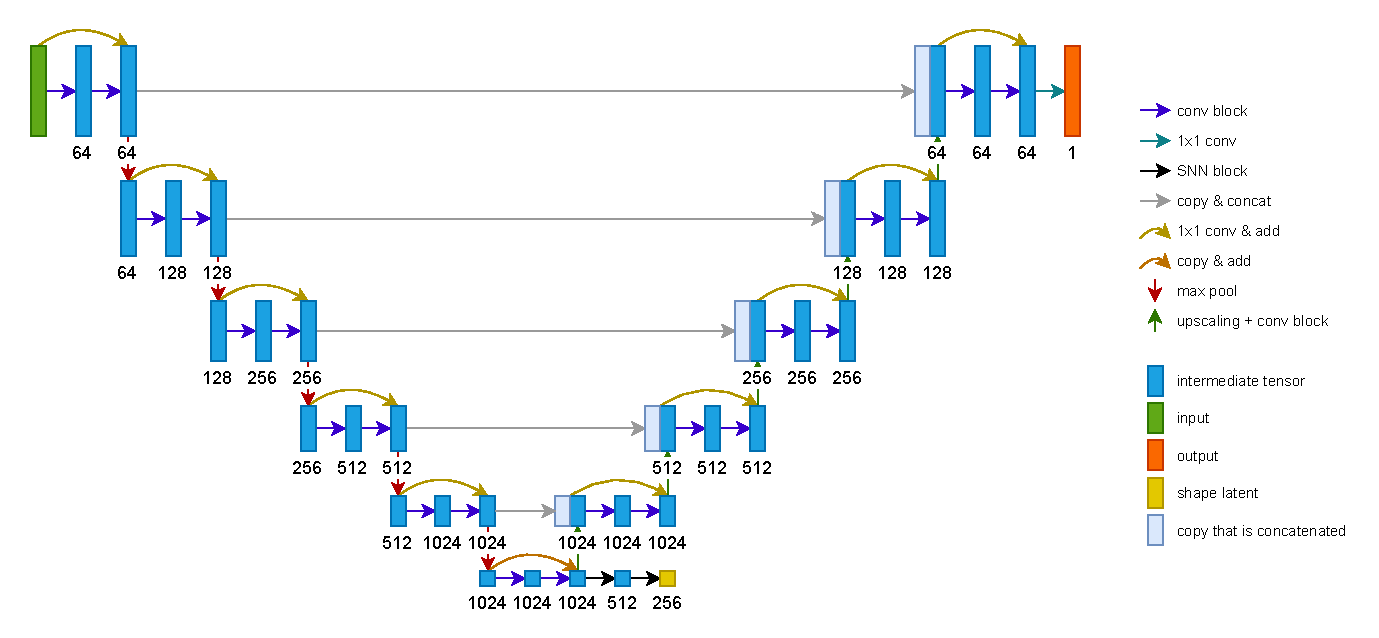
\includegraphics[width=0.9\textwidth]{images/CIL-arch.pdf}
    \caption{The model's architecture}%
    \label{fig:arch}
\end{figure*}
